\documentclass{article}                      
\usepackage{siunitx}                          \usepackage{setspace}                        
\usepackage{gensymb}
\usepackage{xcolor}                           \usepackage{caption}                          %\usepackage{subcaption}                      %\doublespacing
\singlespacing
\usepackage[none]{hyphenat}                   \usepackage{amssymb}
%\usepackage{relsize}
\usepackage[cmex10]{amsmath}                  \usepackage{mathtools}                        \usepackage{amsmath}
\usepackage{commath}
%\usepackage{amsthm}
%\interdisplaylinepenalty=2500                %\savesymbol{iint}                            %\usepackage{txfonts}
%\restoresymbol{TXF}{iint}
%\usepackage{wasysym}                         \usepackage{amsthm}                           \usepackage{mathrsfs}
\usepackage{txfonts}
\let\vec\mathbf{}
%\usepackage{stfloats}
\usepackage{float}
\usepackage{cite}
\usepackage{cases}
\usepackage{subfig}                           %\usepackage{xtab}                            \usepackage{longtable}
\usepackage{multirow}
%\usepackage{algorithm}
\usepackage{amssymb}                          %\usepackage{algpseudocode}
\usepackage{enumitem}
\usepackage{mathtools}
%\usepackage{eenrc}
%\usepackage[framemethod=tikz]{mdframed}      \usepackage{listings}                         \usepackage{listings}                         \usepackage[latin1]{inputenc}                 %% \usepackage{color}
\usepackage{titling}
%\usepackage{fulbigskip}
\usepackage{tikz}                             \usepackage{graphicx}
\begin{document}
\title{CLASS 12\\DIFFERENTIATION}
\date{}
\maketitle
\section{EXERCISE 1}
\begin{enumerate}
	\item If $\tan{{x+y}\over{x-y}}=k$,then $\dfrac{dy}{dx}$ is equal to 
		\begin{enumerate}
			\item ${{-y}\over{x}}$
			\item ${{y}\over{x}}$
			\item $\sec^2{{y}\over{x}}$
			\item $\-sec^2{{y}\over{x}}$
		\end{enumerate}
\item  \textbf{Assertion(A) :}Maximum value of $({\cos^{-1}})^2$ is ${{\pi}^2}$.\\
  \textbf{Reason(R):}Range of the principle value branch of ${{\cos^{-1}x}}$ is $[{\frac{\pi}{2}},{\frac{\pi}{2}}]$.\\
	\item If y=$\sqrt{ax+b}$ , prove that $y(\dfrac{d^2y}{dx^2})+(\dfrac{dy}{dx})^2=0$ \\
 \item If the circumference of circle is increasing at the constant rate, prove that rate of change of area of circle is directly proportional to its radius.
 \item Engine displacement is the measure of the cylinder volume swept by all the pistons of a piston engine.The piston moves inside the cylinder bore
 
     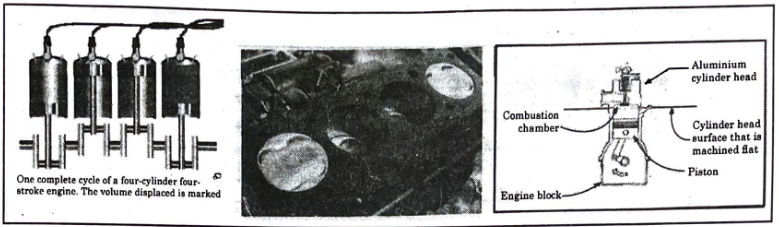
\includegraphics[width=.7\textwidth,height=.7\textheight,keepaspectratio]{figs/engine.png}
    \vspace{0.5cm}
 
 The cylinder bore in the form of circular cylinder open at the top is to be made from a metal sheet of area ${75\pi}$ ${cm}^2.$
 \vspace{1.0cm}
 Based on the above information , answer the following questions:
 \begin{itemize}
     \item[(i)]  If tthe radius of cylinder is r cm and height is h cm, then write the volume V of cylinder in terms of radius r. \hspace{7.3cm} \textbf{1}
     \item[(ii)] Find $\dfrac{dv}{dr}.$\hspace{10.5cm}\textbf{1}
     \item[(iii)] (a) Find the radius of cylinder when its volume is maximum. \hspace{1.6cm}\textbf{2}\\
     \centering \textbf{OR}\\
     (b) For maximum volume, $h > r$.State true or false and justify. \hspace{1.2cm}\textbf{2}
 \end{itemize}
 \item The use of electric vehicles will curb air pollution in the long run.
 
 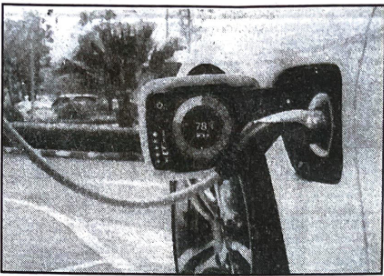
\includegraphics[width=.7\textwidth,height=.7\textheight,keepaspectratio]{figs/electricvehicle.png}
  \hspace{10.5cm}
  \vspace{0.2cm}
 The The use of electric vehicles is increasing every year and estimated electric vehicles in use at any time t is given by the function V :\\
 \vspace{0.4cm}
 \hspace{0.2cm}V(t)=$\frac{1}{5}t^3 - \frac{5}{2}t^2 + 25t-2$ \\
 Where t represents the time and t=1,2,3.... corresponds to year 2001,2002,2003,.....respectively.\\ \vspace{0.3cm}
 Based on the above information, answer the following questions :
 \begin{enumerate}
     \item[i] Can the above function be used to estimate number of vehicles in the year 2000 ? Justify. \hspace{10.3cm} \textbf{2}
     \item[ii] Prove that the function V(t) is an increasing function. \hspace{5.0cm} \textbf{2}
 \end{enumerate}
  \end{enumerate}
  \end{document}



